
% Our goal is to demonstrate that regularisation makes robotic policies more resilient to the sim-to-real gap.
% We introduced \ourMethod to provide a more robust alternative to entropy-regularised policies.
% While \autoref{sec:mujoco} demonstrates that \ourMethod can learn competitive policies in simulation, the question of real-world robustness remains.
% This section evaluates the real-world performance of learned policies, both under nominal deployment conditions and under conditions that differ from those seen in training.
% Robotics provides a direct test of this setting: the sim-to-real gap is, by construction, a deployment-time distribution shift.
% We therefore evaluate how regularisation can improve real-world policy deployment by 1) reducing the performance degradation caused by such shifts in \autoref{sec:robotic_nominal}; and 2) improving robustness to deployment-time perturbations on physical robots in \autoref{sec:robotic_perturb}.
% Our results demonstrate that regularised methods outperform unregularised methods in sim-to-real transfer and perturbation robustness in a majority of tasks.
\vspace{-6pt}
Our goal is to test whether regularisation makes robotic policies more robust to the sim-to-real gap and to perturbations after deployment. While \autoref{sec:mujoco} demonstrates that \ourMethod learns competitive policies in simulation, the question of real-world transfer robustness remains. 
In this section, we deploy policies trained in simulation on two robots. 
% We first evaluate them without modifying the real-world setup. 
% We then modify one aspect of the deployment setup at a time, such as sensor noise, object mass, or surface friction.
We begin with evaluation on a simulation-to-real matched setup, then perturb individual deployment parameters (sensor noise, object mass, surface friction) to
 assess robustness under domain shift.
\autoref{sec:robotic_nominal} evaluates sim-to-real transfer, and \autoref{sec:robotic_perturb} evaluates robustness to these deployment-time perturbations.
\ourMethod achieves the highest return under every perturbation we tested, supporting our hypothesis that regularised policies would be the most robust to the sim-to-real gap and perturbations.

\subsection{Experimental setup}
\label{sec:robotic_setup}


% \textbf{Tasks and platforms.} We evaluate four tasks across two robotic platforms: a manipulator and a quadruped. On the Franka Emika Panda manipulator, Reach requires moving the end effector to a target pose, while Lift requires grasping a cube and lifting it to a target position.
% On an ANYmal-D quadruped, we evaluate velocity tracking on flat and rough terrain.
% The flat-terrain policy is blind to exteroceptive information, whereas the rough-terrain policy receives perceptual observations.
% Policies are trained in the corresponding \texttt{Isaac-Reach-Franka-v0}, \texttt{Isaac-Lift-Cube-Franka-v0}, \texttt{Isaac-Velocity-Flat-Anymal-D-v0}, and \texttt{Isaac-Velocity-Rough-Anymal-D-v0} environments using the default randomisation ranges specified in \aref{sec:isaac_dr}.
% \autoref{fig:robot_setup} shows the four deployment settings.

\textbf{Tasks and platforms}. We evaluate four tasks with two robots: a manipulator and a quadruped. On the Franka Panda arm, the Reach task requires moving the end effector to a target pose, while the Lift task requires grasping a cube and lifting it to a target position. On an ANYmal-D quadruped, we evaluate velocity tracking on flat and rough terrains.
The flat-terrain policy is blind to exteroceptive information, whereas the rough-terrain policy receives perceptual observations. Policies are trained in the corresponding \texttt{Isaac-Reach-Franka-v0}, \texttt{Isaac-Lift-Cube-Franka-v0}, \texttt{Isaac-Velocity-Flat-Anymal-D-v0}, and \texttt{Isaac-Velocity-Rough-Anymal-D-v0} environments using the default DR ranges specified in \aref{sec:isaac_dr}.
\autoref{fig:robot_setup} shows the four deployment settings.



\begin{figure}[t]
\centering
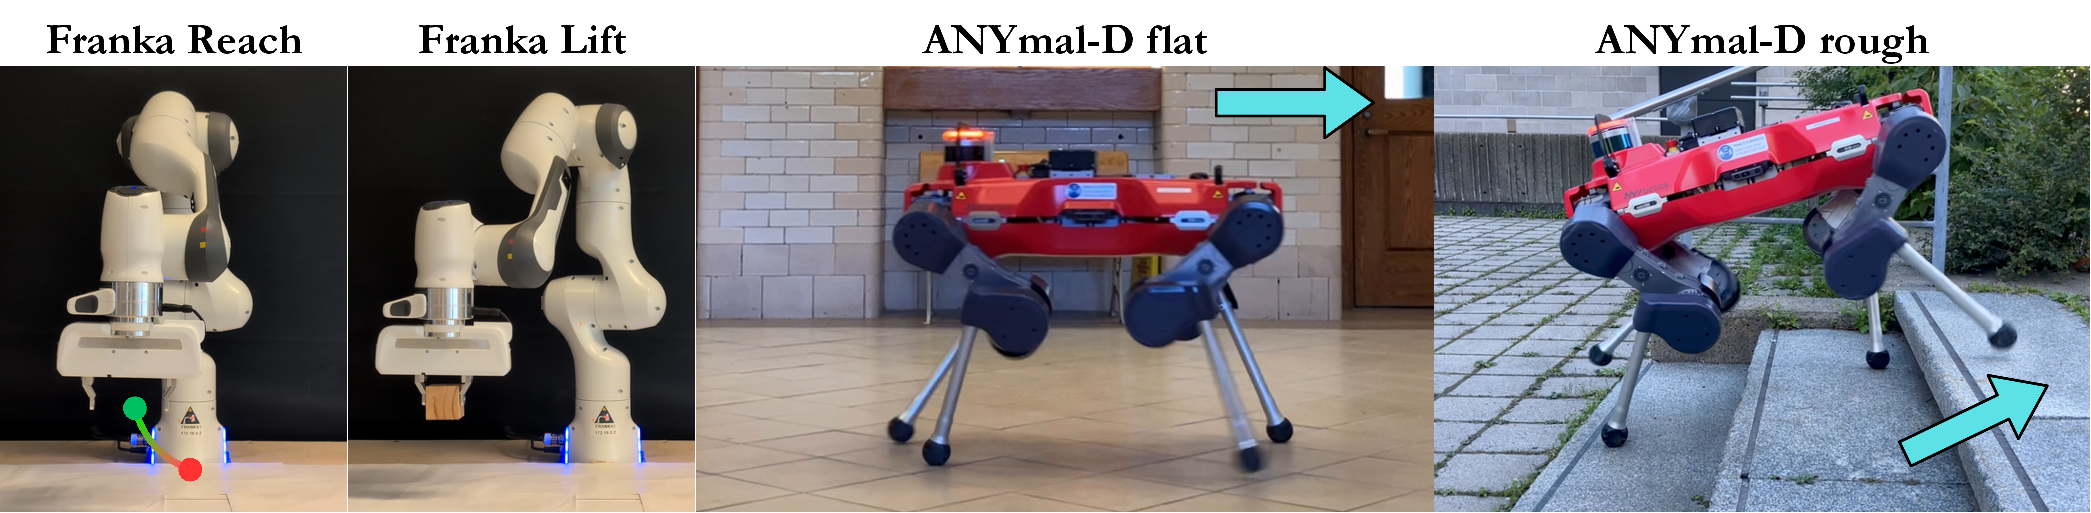
\includegraphics[width=\textwidth]{images/robo_setup.pdf}
\caption{The four real-world evaluation settings: Franka Reach and Lift, and ANYmal-D velocity tracking on flat and rough terrain. For the ANYmal-D tasks, blue arrows indicate the robot's direction of commanded velocity.}
\label{fig:robot_setup}
\end{figure}



\textbf{Algorithms and configurations}.
We compare PPO, FastTD3, SAC, and \ourMethod.
PPO is implemented with RSL-RL \citep{schwarke2025rslrl}, with sweeps over its entropy coefficient, learning rate, target KL, and rollout length.
FastTD3 is a strong unregularised off-policy baseline \citep{seo2025fasttd3}.
We report both at their best configuration per task.
SAC and \ourMethod use the FlashSAC implementation \citep{kim2026flashsac}. We refer to these simply as SAC and \ourMethod below.
For both regularised methods, we fix $\alpha=1$ and sweep $\omega \in \{400,800,1200\}$.
We do not use SAC temperature autotuning, since doing so would remove the controlled variation in regularisation strength that is central to this experiment.
Each configuration is trained with five random seeds.

\textbf{Reward scales}.
The reward functions have substantially different scales across tasks, with a good episode returning roughly $0.7$ on Reach, $150$ on Lift, and $20$ on either ANYmal task.
Because the regularisation term in the value function is scaled by $1/\omega$ (\autoref{equ:regularised_evaluation_funcs}), a fixed inverse temperature induces different effective regularisation strengths across tasks.
We therefore sweep $\omega$ separately for each task and report all three values.


\textbf{Perturbations}.
To test robustness, we perturb task parameters while keeping each trained policy fixed. The policy, command, and low-level controller are unchanged throughout. 
On Franka, we add Gaussian observation noise ($\sigma=0.005$ on Reach, and $\sigma=0.001$ and $\sigma=0.005$ on Lift). On Lift, we additionally use a cube of twice the training mass, or a cube with a $15$mm center-of-mass (CoM) offset. 
On ANYmal, we lower surface friction by deploying on wet concrete, push the base (flat terrain only), add a $7$kg payload, and add Gaussian noise ($\sigma=0.001$) to the proprioceptive inputs at every step. For safety reasons, a configuration is deployed under a perturbation only if it fails fewer than $80\%$ of simulated episodes under the same perturbation. This rule is fixed in advance and applied to every configuration. As a result, PPO and FastTD3 are excluded from all ANYmal perturbation experiments.
These perturbations are similar to \citet{danesh2025safe}, who evaluate ANYmal-D on surfaces with different friction and with a $3$kg payload.


\textbf{Metrics}.
% We report overall episode return for all tasks.
% For Franka, we additionally report the distance between the end effector or cube and the target pose at the end of the episode.
% For ANYmal, we report the root mean squared error (RMSE) between commanded and measured base velocity.
% An ANYmal episode is considered successful if the robot remains upright for the full $20$-second episode.
% Returns and errors are averaged over seeds. And success is evaluated at the seed level.
We report the mean and one standard deviation of the episode return across seeds. \autoref{tab:robot_returns} lists the return of every configuration without perturbation and under each perturbation. \autoref{fig:robot_retention} shows the return under each perturbation as a percentage of the same configuration's return without it. Therefore, a value of $100\%$ indicates that the perturbation incurs no performance cost. Note that values slightly above $100\%$ indicate no loss rather than an improvement. In \aref{sec:robot_appendix}, we additionally report the task error without perturbation (\autoref{tab:robot_nominal}), measured as the distance between the end effector or cube and the target at the end of the episode for Franka, and as the root mean squared error between commanded and measured base velocity for ANYmal.
An ANYmal episode is considered successful if the robot remains upright for the full $20$-second episode.


% \begin{table}[t]
% \centering
% \caption{Nominal deployment on hardware. PPO and FastTD3 are shown at their best configurations per task. Bold entries indicate the best mean within each metric and task.}
% \label{tab:robot_nominal}
% \setlength{\tabcolsep}{4pt}
% \resizebox{\textwidth}{!}{\begin{tabular}{llcccccccc}
% \toprule
% & & \multicolumn{2}{c}{Reach} & \multicolumn{2}{c}{Lift} & \multicolumn{2}{c}{ANYmal flat} & \multicolumn{2}{c}{ANYmal rough} \\
% \cmidrule(lr){3-4}\cmidrule(lr){5-6}\cmidrule(lr){7-8}\cmidrule(lr){9-10}
% Agent & $\omega$ & err (cm) & ret. & err (cm) & ret. & RMSE (m/s) & ret. & RMSE (m/s) & ret. \\
% \midrule
% PPO & --- &
% \textbf{0.64} \sd{0.11} & \textbf{0.69} \sd{0.04} &
% 5.79 \sd{3.6} & 133.10 \sd{54.75} &
% 0.2289 \sd{0.047} & 18.94 \sd{5.55} &
% 0.5775 \sd{0.081} & 8.60 \sd{3.66} \\
% FastTD3 & --- &
% 0.93 \sd{0.14} & 0.40 \sd{0.09} &
% 4.26 \sd{0.6} & 123.14 \sd{4.05} &
% 0.1955 \sd{0.018} & 23.60 \sd{0.70} &
% 0.5295 \sd{0.073} & 13.72 \sd{4.13} \\
% \midrule
% \multirow{3}{*}{SAC}
% & 400 &
% 0.93 \sd{0.16} & 0.48 \sd{0.12} &
% 16.53 \sd{9.4} & 92.90 \sd{83.80} &
% 0.1439 \sd{0.012} & 25.28 \sd{0.28} &
% 0.3689 \sd{0.044} & 19.11 \sd{1.62} \\
% & 800 &
% 0.79 \sd{0.12} & 0.58 \sd{0.09} &
% 8.54 \sd{7.1} & 125.78 \sd{69.93} &
% 0.1369 \sd{0.010} & 25.18 \sd{0.45} &
% 0.3471 \sd{0.057} & 19.33 \sd{4.90} \\
% & 1200 &
% 0.91 \sd{0.15} & 0.53 \sd{0.09} &
% 17.32 \sd{9.7} & 94.93 \sd{86.04} &
% 0.1355 \sd{0.009} & 24.77 \sd{0.09} &
% 0.3386 \sd{0.049} & 18.78 \sd{3.40} \\
% \midrule
% \multirow{3}{*}{\ourMethod (ours)}
% & 400 &
% 1.00 \sd{0.15} & 0.51 \sd{0.08} &
% 1.53 \sd{0.6} & 148.48 \sd{8.61} &
% 0.1509 \sd{0.011} & 24.98 \sd{0.42} &
% 0.4112 \sd{0.045} & 20.96 \sd{1.18} \\
% & 800 &
% 0.76 \sd{0.10} & 0.61 \sd{0.03} &
% \textbf{0.82} \sd{0.2} & \textbf{152.87} \sd{2.52} &
% \textbf{0.1268} \sd{0.008} & \textbf{25.89} \sd{0.40} &
% 0.3252 \sd{0.038} & 20.82 \sd{1.32} \\
% & 1200 &
% 1.07 \sd{0.17} & 0.45 \sd{0.05} &
% 8.57 \sd{6.6} & 123.94 \sd{69.39} &
% 0.1523 \sd{0.012} & 25.51 \sd{0.30} &
% \textbf{0.2938} \sd{0.034} & \textbf{21.93} \sd{1.60} \\
% \bottomrule
% \end{tabular}}
% \end{table}

% \begin{table}[t]
% \centering
% \caption{Robustness under deployment-time perturbations. Retention is perturbed return as \% of nominal (100\% = no loss). ``---'' = excluded by safety screen. \textbf{Bold} = best per column. \ourMethod retains more return than all baselines in every condition tested.}
% \label{tab:robot_retention}
% \setlength{\tabcolsep}{4pt}
% \resizebox{\textwidth}{!}{\begin{tabular}{llccccccc}
% \toprule
% & & \multicolumn{2}{c}{Reach} & \multicolumn{3}{c}{Lift} & \multicolumn{2}{c}{ANYmal (flat / rough)} \\
% \cmidrule(lr){3-4}\cmidrule(lr){5-7}\cmidrule(lr){8-9}
% Agent & $\omega$ & nominal ret. & obs.\ noise & nominal ret. & 2$\times$mass & CoM shift & nominal ret. & avg.\ retention \\
% \midrule
% PPO & --- &
% \textbf{0.69} & 15--29\% &
% 133 & 73\% & 89\% &
% 18.9 / 8.6 & --- \\
% FastTD3 & --- &
% 0.40 & 59--78\% &
% 123 & --- & --- &
% 23.6 / 13.7 & --- \\
% \midrule
% \multirow{3}{*}{SAC}
% & 400 &
% 0.48 & 54\% &
% 93 & --- & --- &
% 25.3 / 19.1 & 87--95\% / 86--93\% \\
% & 800 &
% 0.58 & 67\% &
% 126 & --- & --- &
% 25.2 / 19.3 & 87--95\% / 86--93\% \\
% & 1200 &
% 0.53 & 87\% &
% 95 & --- & --- &
% 24.8 / 18.8 & 87--95\% / 86--93\% \\
% \midrule
% \multirow{3}{*}{\ourMethod (ours)}
% & 400 &
% 0.51 & 74\% &
% 148 & 99\% & 104\% &
% 25.0 / 21.0 & 95--101\% / 88--102\% \\
% & 800 &
% \textbf{0.61} & \textbf{92\%} &
% \textbf{153} & \textbf{102\%} & \textbf{102\%} &
% \textbf{25.9} / 20.8 & \textbf{95--101\%} / \textbf{100--102\%} \\
% & 1200 &
% 0.45 & 98\% &
% 124 & 100\% & 102\% &
% 25.5 / \textbf{21.9} & 95--101\% / 88--102\% \\
% \bottomrule
% \end{tabular}}
% \end{table}




\begin{table}[t]
\centering
\caption{Return on hardware with and without perturbations.
Entries are the mean and one standard deviation of the return across seeds. Each column is one trained configuration, and reading down a column within a task shows how its return changes under each perturbation. The \textit{none} row is the deployment without perturbation. PPO and FastTD3 are shown at their best configuration per task. \colorbox{highlight}{Highlighted} entries indicate the highest return in each row. Entries marked with ``---'' were not deployed, because the configuration failed the simulation safety check  (\autoref{sec:robotic_setup}). Task errors for the \textit{none} rows are reported in \autoref{tab:robot_nominal}.}
\label{tab:robot_returns}
\small
\setlength{\tabcolsep}{4pt}
\resizebox{\textwidth}{!}{\begin{tabular}{lcccccccc}
\toprule
 & & & \multicolumn{3}{c}{SAC} & \multicolumn{3}{c}{\ourMethod (ours)} \\
\cmidrule(lr){4-6}\cmidrule(lr){7-9}
Perturbation & PPO & FastTD3 & $\omega{=}400$ & $800$ & $1200$ & $\omega{=}400$ & $800$ & $1200$ \\
\midrule
\multicolumn{9}{l}{\textit{Franka Reach}} \\
none & \cellcolor{highlight}0.69 \sd{0.04} & 0.40 \sd{0.09} & 0.48 \sd{0.12} & 0.58 \sd{0.09} & 0.53 \sd{0.09} & 0.51 \sd{0.08} & 0.61 \sd{0.03} & 0.45 \sd{0.05} \\
\quad obs.\ noise ($\sigma{=}0.005$) & 0.19 \sd{0.05} & 0.24 \sd{0.03} & 0.35 \sd{0.03} & 0.40 \sd{0.03} & 0.35 \sd{0.02} & 0.45 \sd{0.02} & \cellcolor{highlight}0.56 \sd{0.02} & 0.33 \sd{0.01} \\
\midrule
\multicolumn{9}{l}{\textit{Franka Lift}} \\
none & 133.1 \sd{54.8} & 123.1 \sd{4.1} & 92.9 \sd{83.8} & 125.8 \sd{69.9} & 94.9 \sd{86.0} & 148.5 \sd{8.6} & \cellcolor{highlight}152.9 \sd{2.5} & 123.9 \sd{69.4} \\
\quad cube mass $2\times$ & 97.5 \sd{11.0} & 102.9 \sd{9.5} & 81.9 \sd{5.2} & 99.1 \sd{4.4} & 87.1 \sd{5.4} & \cellcolor{highlight}152.5 \sd{9.1} & 151.6 \sd{3.1} & 128.3 \sd{8.2} \\
\quad CoM offset ($15$\,mm) & 118.2 \sd{5.6} & 106.8 \sd{3.9} & 93.4 \sd{4.5} & 115.0 \sd{7.8} & 96.2 \sd{5.9} & \cellcolor{highlight}154.4 \sd{9.2} & 153.0 \sd{2.8} & 127.6 \sd{10.3} \\
\quad obs.\ noise ($\sigma{=}0.001$) & 38.0 \sd{8.4} & 96.5 \sd{3.0} & 81.1 \sd{4.8} & 103.4 \sd{11.6} & 82.1 \sd{5.5} & 147.0 \sd{3.1} & \cellcolor{highlight}150.2 \sd{2.3} & 122.4 \sd{2.5} \\
\quad obs.\ noise ($\sigma{=}0.005$) & 19.4 \sd{9.2} & 72.4 \sd{5.7} & 60.7 \sd{7.2} & 68.5 \sd{7.8} & 62.5 \sd{6.6} & \cellcolor{highlight}120.9 \sd{12.2} & \cellcolor{highlight}120.9 \sd{4.0} & 107.7 \sd{4.6} \\
\midrule
\multicolumn{9}{l}{\textit{ANYmal flat}} \\
none & 18.9 \sd{5.6} & 23.6 \sd{0.7} & 25.3 \sd{0.3} & 25.2 \sd{0.5} & 24.8 \sd{0.1} & 25.0 \sd{0.4} & \cellcolor{highlight}25.9 \sd{0.4} & 25.5 \sd{0.3} \\
\quad low friction & --- & --- & 22.3 \sd{1.3} & 22.5 \sd{1.1} & 21.5 \sd{1.5} & 24.5 \sd{0.2} & \cellcolor{highlight}24.7 \sd{0.4} & 24.6 \sd{0.3} \\
\quad push & --- & --- & 23.0 \sd{1.2} & 22.8 \sd{1.0} & 21.8 \sd{1.4} & \cellcolor{highlight}25.3 \sd{0.2} & \cellcolor{highlight}25.3 \sd{0.3} & 24.9 \sd{0.3} \\
\quad payload & --- & --- & 24.1 \sd{0.7} & 22.6 \sd{1.1} & 22.8 \sd{0.9} & 25.1 \sd{0.2} & \cellcolor{highlight}25.2 \sd{0.3} & 25.0 \sd{0.2} \\
\quad proprioceptive noise & --- & --- & 20.7 \sd{2.2} & 20.5 \sd{2.0} & 20.5 \sd{1.9} & \cellcolor{highlight}24.7 \sd{0.2} & \cellcolor{highlight}24.7 \sd{0.4} & \cellcolor{highlight}24.7 \sd{0.3} \\
\midrule
\multicolumn{9}{l}{\textit{ANYmal rough}} \\
none & 8.6 \sd{3.7} & 13.7 \sd{4.1} & 19.1 \sd{1.6} & 19.3 \sd{4.9} & 18.8 \sd{3.4} & 21.0 \sd{1.2} & 20.8 \sd{1.3} & \cellcolor{highlight}21.9 \sd{1.6} \\
\quad low friction & --- & --- & 16.4 \sd{1.5} & 17.0 \sd{0.8} & 17.4 \sd{1.0} & 18.5 \sd{0.6} & 21.2 \sd{0.6} & \cellcolor{highlight}21.9 \sd{1.1} \\
\quad payload & --- & --- & 17.2 \sd{0.6} & 16.8 \sd{0.9} & 16.8 \sd{1.9} & 21.2 \sd{0.8} & 20.5 \sd{0.5} & \cellcolor{highlight}21.5 \sd{1.1} \\
\quad proprioceptive noise & --- & --- & 15.3 \sd{1.6} & 15.3 \sd{1.9} & 13.5 \sd{1.0} & 18.8 \sd{1.4} & \cellcolor{highlight}19.3 \sd{0.7} & 18.9 \sd{1.9} \\
\bottomrule
\end{tabular}}
\end{table}

\subsection{Sim-to-real transfer}
\label{sec:robotic_nominal}
% \john{I would remove the reach results and focus on the lift instead. people can look at the table for the results I don't think we need to address that explicitly It's gonna open for criticism}
% On Reach, PPO achieves the lowest error and highest return.
% This contact-free task is comparatively well modelled in simulation, so the additional stochasticity associated with regularised policies is not necessary to solve the task and can come with a performance cost \citep{zhang2025when}.
% This provides an important counterexample to a blanket claim that stronger regularisation should improve transfer.

% \john{I would highlight these results a lot more more positive statement also the table with the results is never cited}
% For a slightly more complex manipulation task which is not contact-free, the picture changes.
% On Lift, \ourMethod at $\omega=800$ achieves the lowest task error and highest return among the deployed configurations.
% It also has substantially lower variability than the SAC configurations.
% The large standard deviations of PPO and SAC indicate that nominal transfer is inconsistent across seeds, whereas the $\omega=800$ \ourMethod configuration is comparatively consistent.

% The same qualitative pattern appears in locomotion.
% On flat terrain, the regularised methods achieve lower velocity-tracking error and higher return than PPO.
% On rough terrain, the gap is larger: \ourMethod at $\omega=1200$ has the lowest velocity-tracking error and highest return among the evaluated configurations.
% These results motivate the perturbation experiments below: nominal transfer alone does not establish whether the apparent advantage of regularisation reflects robustness or simply a better nominal solution.

\textbf{\ourMethod transfers best on Lift and both locomotion tasks.}
The \textit{none} rows of \autoref{tab:robot_returns} report the return of each policy deployed without perturbation. In locomotion, every regularised configuration achieves a higher return that PPO and FastTD3 on both terrains, with the largest gap on rough terrain. 
On Lift, the two best configurations are both \ourMethod.
The best of these, at $\omega=800$, is also far more consistent across seeds than PPO and SAC, whose large standard deviations indicate that their transfer varies considerably from seed to seed.

\textbf{Regularised policies remain deployable under a larger sim-to-real gap.}
We further widen the sim-to-real gap by limiting domain randomisation in training (\aref{sec:isaac_dr}) and deploying the resulting policies on hardware (\aref{sec:robot_dr_appendix}).
Limiting domain randomisation lowers the return of every method, indicating that DR remains important for regularised policies as well.
On ANYmal, however, PPO and FastTD3 no longer pass the simulation safety check once the randomisation is limited, and are thus not deployable.
On Lift, \ourMethod achieves the highest return at every DR level.
Regularisation and DR thus appear complementary, since limiting the randomisation hurts every method, while regularised policies remain deployable where unregularised ones are not.

% However, sim-to-real transfer alone does not establish whether this advantage reflects robustness or simply better performance under the training conditions. The perturbation experiments below investigate this distinction.



\subsection{Robustness to deployment-time perturbations}
\label{sec:robotic_perturb}

\begin{figure}[t]
\centering
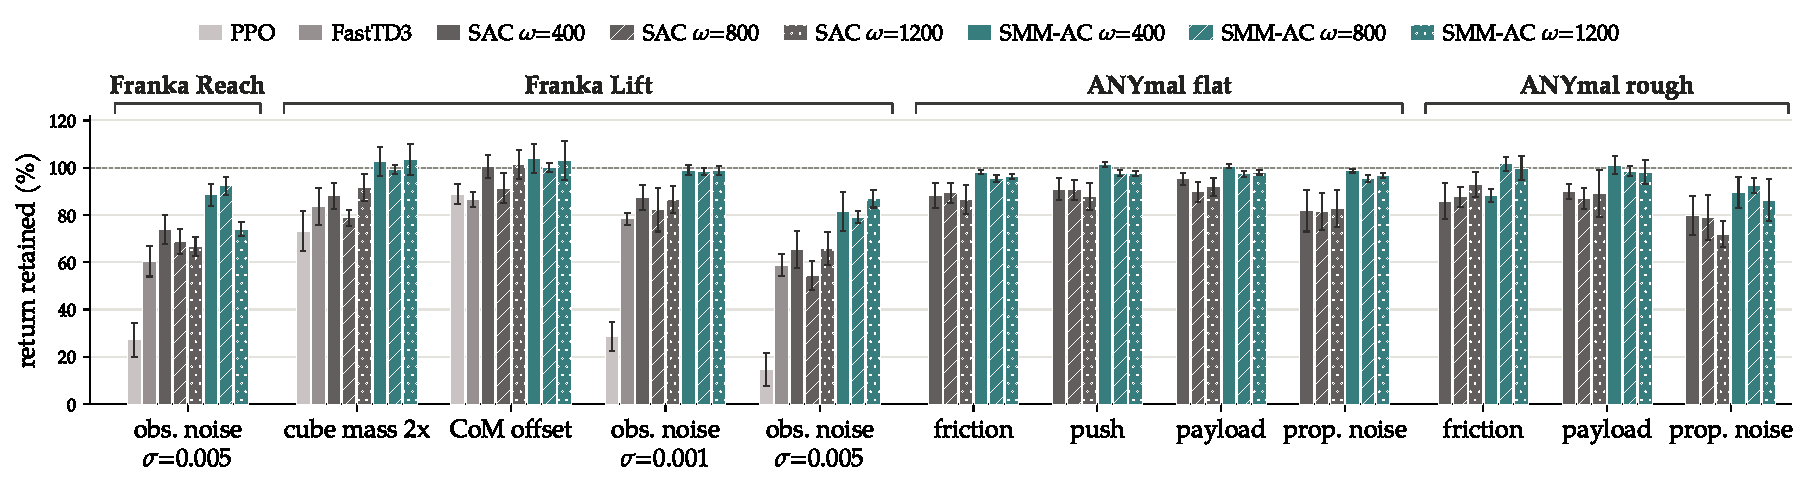
\includegraphics[width=\textwidth]{images/robot_retention.pdf}
\caption{Return kept under real-world deployment-time perturbations. Return under each perturbation as a percentage of the same configuration's return without it, so $100\%$ means no loss. Bars are seed means, and error bars show one standard deviation. Franka is perturbed with Gaussian observation noise and, on Lift, with a cube of 2$\times$ the training mass and with a $15$mm CoM offset. ANYmal is perturbed with lower surface friction, pushes, a payload, and proprioceptive noise. PPO and FastTD3 do not appear on ANYmal because they fail the simulation safety check, which is applied identically to every configuration.}
\label{fig:robot_retention}
\end{figure}



% Nominal 
% \john{I'm not sure I like the word nominal. It doesn't seem to be adding a lot And it makes the sentence confusing to me. Maybe it's just me. Nominal means existing in name only, very small in cost, or relating to a name, a noun, or unadjusted financial figures} \hc{let's come up with a few names: in-distribution transfer?}
% transfer alone does not reveal how policies respond to changes in deployment conditions after training. We therefore keep each trained policy fixed, change one aspect of the physical deployment, and measure how much of the original return survives (\autoref{fig:robot_setup}).

% \textbf{Setup.}
% On Franka, we add Gaussian observation noise ($\sigma=0.005$ on Reach; $\sigma=0.001$ and $\sigma=0.005$ on Lift) and, separately on Lift, use a cube of twice the training mass or with a $15$mm CoM offset.
% On ANYmal, we lower surface friction by deploying on wet concrete, push the base, add a $7$kg payload, and add Gaussian observation noise ($\sigma=0.001$) to the proprioceptive measurements at every control step.
% The policy, command, and controller are unchanged throughout.
% We report retained return, $R_{\mathrm{ret}} = 100\, R_{\mathrm{perturbed}}/R_{\mathrm{nominal}}$, where both terms are seed averages of the same configuration, so $100\%$ means the perturbation cost nothing and slightly higher values mean no loss rather than an improvement.
% A configuration is deployed only if it fails fewer than $80\%$ of simulated episodes under identical perturbations. This rule is fixed in advance, applied to every configuration, and excludes PPO and FastTD3 from all ANYmal perturbations.
% A missing bar therefore means ``not deployed'', not ``deployed and failed''.
% \hc{Are those inside/outside of the default randomization range? Did you randomize Gaussian observation noise during training? }
% \hc{refer to fig 4}


% \textbf{\ourMethod loses the least in every condition.}
% At matched temperature it retains more of its nominal return than SAC in all twelve conditions, in $29$ of those $36$ comparisons by more than the two standard deviations combined.
% Averaged over conditions and temperatures it keeps $96\%$ of its nominal return against $84\%$ for SAC, with about half the spread, and it retains more than PPO and FastTD3 wherever those were deployed.
% How much a policy loses, however, depends mostly on which perturbation it faces.


% \textbf{Observation noise causes the largest losses.}
% On Franka, PPO keeps $15-29\%$ of its return and FastTD3 $59-78\%$, against $54-87\%$ for SAC and $74-99\%$ for \ourMethod.
% Proprioceptive noise on ANYmal is likewise the perturbation that separates the two regularised methods most, with SAC at $72-83\%$ and \ourMethod at $86-99\%$.
% Since the dynamics are untouched, these losses come entirely from how each policy responds to corrupted inputs.

% \textbf{Changes to the physical system cost less.}
% With a heavier or unbalanced cube, PPO retains $73-89\%$ and \ourMethod loses nothing ($99-104\%$), so robustness is specific to the perturbation rather than a single property of a policy.
% Under the ANYmal contact perturbations, \ourMethod retains $95-101\%$ on flat terrain and $88-102\%$ on rough, against $87-95\%$ and $86-93\%$ for SAC.
% While flat terrain is insensitive to the temperature, rough terrain is not, where \ourMethod retains $88\%$ under the friction change at $\omega=400$ but $100-102\%$ at $\omega=800$ and $1200$.
% \hc{i am not sure if "changes to the physical system" really describes the outcome above}

% \textbf{Retention is not performance.}
% Multiplying retention by nominal return (\autoref{tab:robot_nominal}) gives what each configuration achieves under perturbation.
% PPO has the best nominal Reach return ($0.69$) but retains only $27\%$ under noise, ending at $0.19$, the lowest of any configuration, while \ourMethod at $\omega=800$ ends at $0.56$.
% On Lift and both ANYmal tasks, every \ourMethod configuration ends above every baseline configuration, so its high retention is not the result of preserving a small return, but rather of maintaining a high absolute level of performance under perturbations.

% \textbf{Discussion.}
% These experiments separate two effects that are easy to conflate: \textit{transferring well to nominal hardware, and keeping that performance as conditions move away from training}.
% Regularisation specifically helps with the second, most clearly on Lift and rough terrain, where the best nominal \ourMethod configuration also keeps nearly all of its return.
% However, this conclusion is not uniformly applicable to all cases. PPO transfers best on nominal Reach, and the advantage of regularisation is largest under observation noise.





% We now change the deployment one aspect at a time and measure how much of its return each policy keeps (\autoref{fig:robot_retention}). 
We now perturb task parameters and report the resulting return as a percentage of its unperturbed return in \autoref{fig:robot_retention}.
%how much of its return each policy retains (\autoref{fig:robot_retention}).
\autoref{tab:robot_returns} reports the corresponding absolute returns.

\textbf{\ourMethod keeps more of its return than the baselines.}
At the same $\omega$, \ourMethod keeps more of its return than SAC under every perturbation, in most cases by more than two standard deviations combined.
It retains more than PPO and FastTD3 wherever those were deployed, in every case by more than the combined standard deviations.
Its results are also more consistent across seeds, with about half the standard deviation of SAC on average. Under most perturbations, \ourMethod loses little or none of its return, while the baselines retain considerably less. However, the empirical drop in performance depends on the type of perturbation.
%empirically, how much a policy loses depends mostly on the type of perturbation.

\textbf{Observation noise causes the largest losses.}
Every method has its largest loss under observation noise, and this is also where the methods differ the most. On Franka, PPO loses most of its return under noise, and FastTD3 and SAC lose a substantial part of theirs. Nevertheless, \ourMethod keeps most of its return.
On ANYmal, proprioceptive noise separates SAC and \ourMethod more than any change to the physical system. Since the dynamics are untouched, these losses come entirely from how each policy responds to corrupted inputs.

\textbf{Changes to the physical system cost less.}
A heavier or unbalanced cube costs \ourMethod nothing, while baselines lose part of their returns.
On ANYmal, \ourMethod loses little under lower friction, pushes, and payload on either terrain, while SAC loses noticeably more.
The one exception is lower friction on rough terrain at $\omega=400$ where \ourMethod loses about as much as SAC. At other values of $\omega$, it loses nothing.

\textbf{\ourMethod maintains the highest absolute return.}
Note that a policy with a low return can still keep a high percentage of it. Therefore, \autoref{tab:robot_returns} reports absolute returns as well. 
Under every perturbation, the highest return in achieved by \ourMethod.
On Lift and locomotion tasks, every configuration of \ourMethod outperforms every deployed baseline under every perturbation.
On Reach, under observation noise, \ourMethod at $\omega=800$ achieves the highest return and PPO the lowest.

\textbf{Discussion.}
These experiments separate two effects that are easy to conflate, namely transferring well to hardware, and keeping that performance as conditions move away from training.
Regularisation helps most clearly with the second.
Across all perturbations, \ourMethod keeps the most return and achieves the highest absolute return.
Its advantage is largest under observation noise, which every real robot faces to some degree in real-world deployment. These results support our hypothesis that regularisation improves sim-to-real performance and robustness to perturbations. They also empirically validate theoretical robustness claims, providing evidence that SMM, with its larger robust sets, is indeed more robust.